% AI-Based Groundwater Depletion Risk Prediction for Mysuru District
% IEEE Conference Paper — IEEEtran class, double-column
% paper_revision_v2/main.tex
%
% BUILD:
%   pdflatex main.tex
%   bibtex main
%   pdflatex main.tex
%   pdflatex main.tex

\documentclass[conference]{IEEEtran}
\IEEEoverridecommandlockouts

% ------------------------------------------------------------------
% PACKAGES
% ------------------------------------------------------------------
\usepackage{cite}
\usepackage{amsmath,amssymb,amsfonts}
\usepackage{algorithmic}
\usepackage{graphicx}
\usepackage{textcomp}
\usepackage{xcolor}
\usepackage{booktabs}
\usepackage{multirow}
\usepackage{array}
\usepackage{url}
\usepackage{xurl}
\usepackage{hyperref}
% \usepackage{balance}

\hypersetup{
  colorlinks=true,
  linkcolor=black,
  citecolor=black,
  urlcolor=blue
}

\setlength{\textfloatsep}{3pt plus 1pt minus 1pt}
\setlength{\floatsep}{3pt plus 1pt minus 1pt}
\setlength{\intextsep}{3pt plus 1pt minus 1pt}
\setlength{\dbltextfloatsep}{3pt plus 1pt minus 1pt}
\setlength{\dblfloatsep}{3pt plus 1pt minus 1pt}

\def\BibTeX{{\rm B\kern-.05em{\sc i\kern-.025em b}\kern-.08em
    T\kern-.1667em\lower.7ex\hbox{E}\kern-.125emX}}

% ------------------------------------------------------------------
% TITLE / AUTHORS
% ------------------------------------------------------------------
\begin{document}

\title{AI-Based Groundwater Depletion Risk Prediction for Mysuru District
       Using Machine Learning}

\author{%
  \IEEEauthorblockN{\textit{Mohammed Sadiq Shariff \qquad Shumail Ali \qquad Deeksha Prasad S P \qquad Nagashree D}}
  \IEEEauthorblockA{Department of Computer Science and Engineering (Artificial Intelligence and Machine Learning)\\
    Maharaja Institute of Technology, Thandavapura\\
    Mysuru, Karnataka, India\\
    Corresponding Author: \texttt{mohammedsadiqshariff80@gmail.com}}
}

\maketitle

% ------------------------------------------------------------------
% ABSTRACT
% ------------------------------------------------------------------
\begin{abstract}
Groundwater depletion is a critical environmental threat in
semi-arid regions of peninsular India. This paper presents an
exploratory machine-learning framework for predicting groundwater
level (GWL) and classifying depletion risk at manually monitored
wells in Mysuru district, Karnataka.
We assemble longitudinal groundwater records from official CGWB
archive snapshots via the National Water Data Portal (NWDP)---historical
archive (1991--2020) and recent archive (2021--2025)---yielding 4,185
modelling records (1997--2023) across 92 stations in Mysuru district
paired with daily district-averaged rainfall from the NWDP Karnataka
daily rainfall series.
A Historical Gradient Boosting Regressor (HistGBT) trained on
features derived from GWL lags, rolling means, station-historical
statistics, and rainfall accumulation windows predicts the
\emph{next} observed GWL
(horizon: 40--200 days, median 91 days) with
MAE\,=\,1.94\,m, RMSE\,=\,2.96\,m, and R$^2$\,=\,0.547 on
657 held-out test records (November 2019--November 2023).
A companion Random Forest classifier assigns each observation to one
of four depletion-severity classes---No~Depletion, Low, Moderate,
and High---achieving 52.8\% accuracy and macro-F1 of 0.457,
outperforming majority-class (45.8\%) and stratified-dummy (30.4\%)
baselines. High-risk episodes remain the hardest to identify
(F1\,=\,0.33). An interactive web dashboard is provided for
exploratory visualisation; it is not intended as an operational
early-warning tool or a substitute for field measurements.
All results are traceable to archived prediction artefacts and
require independent hydrogeological validation before
operational deployment.
\end{abstract}

\begin{IEEEkeywords}
groundwater level prediction, depletion risk classification,
machine learning, ensemble methods, Mysuru district, CGWB,
temporal validation, exploratory dashboard
\end{IEEEkeywords}

% ------------------------------------------------------------------
\section{Introduction}
\label{sec:intro}
% ------------------------------------------------------------------

Groundwater constitutes a vital natural resource for rural drinking
water supplies and agricultural irrigation across peninsular India.
In Karnataka's Mysuru district---a mixed agricultural and
peri-urban region---seasonal rainfall variability, unregulated
extraction, and heterogeneous aquifer lithology combine to produce
sharp inter-annual fluctuations in the water table.
Official CGWB assessments record \emph{depth to water table}
(metres below ground level, mbgl), where larger values indicate
greater depth and therefore worse groundwater conditions.

\textbf{Research motivation.}
Long monitoring gaps (typically 30--200 days, median 91 days) and
the absence of continuous sensor networks make it difficult to
detect emerging depletion trends in real time.
A data-driven model that estimates the GWL at the time of the
\emph{next scheduled observation} could assist field staff in
prioritising wells and allocating monitoring resources.

\textbf{Research questions.}
\begin{enumerate}
  \item Can GWL at the next observation---a horizon of
        40--200 days---be estimated from historical in-situ
        observations, station characteristics, and
        accumulated rainfall?
  \item Can a magnitude-of-change label (No~Depletion, Low,
        Moderate, High) be predicted reliably enough to support
        exploratory risk screening?
\end{enumerate}

\textbf{Scope and limitations.}
This study covers 92 CGWB monitoring stations within Mysuru
district.
It does not claim district-wide representativeness, live
forecasting capability, or readiness for operational deployment.
Predictions reflect patterns in historical quarterly monitoring
data; they cannot replace hydrogeological field surveys or
CGWB ground-truth assessments.
The risk labels are defined empirically (Section~\ref{sec:target})
and require hydrogeological validation.

The remainder of the paper is organised as follows:
Section~\ref{sec:related} surveys related work;
Section~\ref{sec:data} describes datasets and preprocessing;
Section~\ref{sec:method} presents the methodology;
Section~\ref{sec:setup} details experimental setup;
Section~\ref{sec:results} reports verified results;
Section~\ref{sec:discussion} discusses limitations;
Section~\ref{sec:conclusion} concludes.

% ------------------------------------------------------------------
\section{Related Work}
\label{sec:related}
% ------------------------------------------------------------------

Machine-learning methods for groundwater level (GWL) prediction
have expanded rapidly, encompassing classical ensembles, hybrid
deep architectures, and physics-informed models
(Table~\ref{tab:relwork}).
Boomika \emph{et al.}\ \cite{boomika2026} developed a hybrid
Random Forest--LSTM architecture combined with IoT-based monitoring
for urban Chennai.
Zeydalinejad \emph{et al.}\ \cite{zeydalinejad2026} evaluated
ANN, LSTM, SVR, Random Forest, and wavelet-enhanced models across
hydro-climatic inputs, highlighting performance variations across
wells and seasons.
Shuai \emph{et al.}\ \cite{shuai2026} integrated physical MODFLOW
numerical simulation with deep LSTM networks to constrain predictions
with hydrological dynamics.
Sankaran \emph{et al.}\ \cite{sankaran2026} employed signal
decomposition and adaptive ensemble learning to forecast groundwater
pressures in industrial zones of Tiruppur under climate variability.
Guo \emph{et al.}\ \cite{guo2026} integrated socioeconomic
groundwater withdrawals into deep CNN and ResNet models to predict
basin-scale groundwater storage in the Yellow River Basin.

\textbf{Research gap.}
While these studies demonstrate predictive capability in dense sensor
networks, physical simulations, or industrial basins, key limitations
persist for regional semi-arid settings:
(i) lack of localized depletion-risk classification paired with
a decision-support dashboard;
(ii) reliance on continuous telemetry or complex physical aquifer
parameters that are unavailable in sparse manual monitoring networks;
and (iii) absence of strict chronological validation isolating
future records.
Our work addresses these gaps using 27+ years of longitudinal CGWB
data in Mysuru district, strict chronological splits (70/15/15),
empirical depletion-severity categorization, and an interactive
exploratory dashboard.

\begin{table*}[t]
\caption{Summary of Related Machine-Learning Studies for Groundwater Prediction}
\label{tab:relwork}
\centering
\scriptsize
\setlength{\tabcolsep}{3.0pt}
\renewcommand{\arraystretch}{1.08}
\begin{tabular}{p{0.6cm} p{1.9cm} p{3.6cm} p{2.7cm} p{3.7cm} p{3.9cm}}
\toprule
\textbf{Year} & \textbf{Authors} & \textbf{Paper} & \textbf{Method Used} & \textbf{Key Finding} & \textbf{Limitation / Research Gap} \\
\midrule
2026 & S.~Boomika \emph{et al.} \cite{boomika2026} & An AI-Driven Hybrid Random Forest--LSTM Framework for IoT-Based Groundwater Level Prediction and Sustainable Water Management in Chennai, India & Hybrid RF--LSTM with IoT sensing (depth, rainfall, temperature, soil moisture) & Outperforms standalone models on Chennai urban aquifer (RMSE = 0.38\,m, MAE = 0.29\,m, $R^2 = 0.96$), cutting LSTM RMSE by $\sim$22\%. & Relies on real-time IoT sensor network and soil-moisture telemetry; lacks regional-scale categorical depletion risk screening and decision web tools. \\
\midrule
2026 & N.~Zeydalinejad \emph{et al.} \cite{zeydalinejad2026} & Performance and Limitations of Machine Learning Models for Groundwater Level Prediction Using Hydro-Climatic Variables & ANN, LSTM, SVR, Random Forest, and wavelet transforms; introduced DDTI metric & Across 11 UK wells, validation $R^2$ varied widely ($<0.1$ to $>0.9$) by hydrogeology; 2-month lag optimal; sharp performance drop in summer ($R^2 < 0.1$). & Focuses on hydro-climatic sensitivity and model failure modes in UK basins; does not establish localized categorical depletion-risk screening. \\
\midrule
2026 & G.~Shuai \emph{et al.} \cite{shuai2026} & Accurate Groundwater Level Predictions: Integration of Physics-Driven and Machine Learning Approaches & MOD-LSTM (coupling MODFLOW physical simulation with LSTM) & On 10 wells in North China Plain, 80\% achieved NSE $> 0.75$; reduced RMSE by 0.618\,m vs.\ MODFLOW and 0.280\,m vs.\ pure LSTM; physical model aids interpretability. & Requires detailed hydrogeological parameters, boundary conditions, and MODFLOW grid inputs unavailable in data-sparse fractured rock. \\
\midrule
2026 & H.~Sankaran \emph{et al.} \cite{sankaran2026} & Assessing and Forecasting Groundwater Resources in the Context of Climate Change Using AI Techniques for the Industry Zones in Tiruppur, India & Signal decomposition (ICEEMDAN, VMD) + SMA-LSTM and CNN-LSTM with Adaptive Weighting & In Tiruppur industrial zone, ensemble achieved MAE = 0.267\,m, RMSE = 0.429\,m, $R^2 = 0.948$, NSE = 0.938; CMIP6 scenarios show future climate stress. & Complex signal decomposition and metaheuristic optimization tailored to industrial point wells; does not offer lightweight tabular screening or web UI. \\
\midrule
2026 & S.~Guo \emph{et al.} \cite{guo2026} & Integrating Socioeconomic Withdrawals Into a Deep Learning Framework for High-Resolution Groundwater Storage Prediction in the Yellow River Basin & Deep learning (CNN, ResNet) with groundwater balance and socioeconomic extraction constraints & Downscaled GRACE to 1\,km across Yellow River Basin; balance constraints cut error by 28\% (CNN) and 68\% (ResNet); 81.2\% of 101 wells had $r > 0.7$. & Predicts basin-scale satellite storage anomalies (GWSA) rather than local well-head depth-to-water table; requires socioeconomic withdrawal data. \\
\bottomrule
\multicolumn{6}{p{16.4cm}}{\footnotesize Note: Publication metadata, methods, and findings for cited 2026 studies were directly verified against the published journal articles.}
\end{tabular}
\end{table*}

% ------------------------------------------------------------------
\section{Dataset and Preprocessing}
\label{sec:data}
% ------------------------------------------------------------------

\subsection{Groundwater Data}

Groundwater level records originate from the Central Ground Water Board
(CGWB) manual quarterly monitoring network published via the
National Water Data Portal (NWDP) \cite{cgwb_data}.
The underlying data correspond to two primary portal resources:
\begin{enumerate}\setlength{\itemsep}{1pt}\setlength{\parskip}{0pt}
  \item \textbf{Historical archive (1991--2020):}
        NWDP resource
        \href{https://nwdp.nwic.gov.in/dataset/gwl-manual-quarterly-central-ground-water-board-department/resource/3dacbc24-b45c-4ffe-8099-f69728ca711b}{\texttt{3dacbc24}},
        archived as
        \path{gwl_manual_quarterly_cgwb_ka_1991_2020.csv} ---
        quarterly manual well measurements for Karnataka with
        raw column ``Groundwater Level Quarterly Manual (meter)'' and
        timestamp ``Data Acquisition Time''
        (\texttt{DD-MM-YYYY HH:MM}).
  \item \textbf{Recent archive (2021--2025):}
        NWDP resource
        \href{https://nwdp.nwic.gov.in/dataset/gwl-manual-quarterly-central-ground-water-board-department/resource/7b76b032-99a5-4725-8ab5-125346e7aebf}{\texttt{7b76b032}},
        archived as
        \path{groundwater_karnataka_2021_2025.csv} ---
        maintaining the same schema for recent monitoring years.
\end{enumerate}
\emph{Data provenance note}: While the official NWDP portal URLs
provide the authoritative access point for live CGWB monitoring records,
the experimental results herein are derived from the verified local
training snapshots to guarantee full numerical reproducibility.
Portal and local CSVs are not assumed to be strictly identical without a
full live-pipeline revalidation, so historical record counts are preserved.

Records are filtered to Mysuru district (case-insensitive match on
``mysore'' or ``mysuru'').
After merging, de-duplicating (on station, date, and coordinates),
and removing impossible values (GWL\,$\leq$\,0\,mbgl or invalid
dates), the dataset comprises \textbf{4,185 station-observation
pairs} from \textbf{92 unique stations}.
GWL is expressed in metres below ground level (mbgl);
larger values indicate a deeper water table.

\subsection{Rainfall Data}

Daily rainfall data correspond to the Karnataka manual daily rainfall
dataset hosted on the National Water Data Portal
(\href{https://nwdp.nwic.gov.in/dataset/rainfall-manual-daily-karnataka}{\path{nwdp.nwic.gov.in/.../rainfall-manual-daily-karnataka}})
\cite{nwdp_rainfall}, assembled from a verified local snapshot of 15
multi-year daily CSV files (\path{rainfall_YYYY_YYYY.csv}, 1989--2025)
and filtered to Mysuru district by name matching.
Official portal datasets and local training snapshots are distinguished
to ensure reproducible results.
Daily values are averaged across all district gauges.
A complete daily calendar is constructed between the earliest and
latest available dates.
Missing days within the calendar are \emph{retained as
\texttt{NaN}} and are not imputed to zero, because missing rainfall
records and genuine zero-rainfall days are indistinguishable.
Rolling windows (7, 30, 90, 180, and 365 days) are computed with
\texttt{min\_periods=1} so that early-series values are not wholly
discarded, but the incomplete coverage of missing intervals is
acknowledged as a limitation.
Rainfall features are joined to groundwater observations using a
backward \texttt{merge\_asof} (nearest prior date), so no future
rainfall information enters any feature.

\subsubsection{December 2023 Rainfall Gap}
Inspection of the assembled rainfall series identifies a data gap in
the December 2023 period corresponding to the final months of the
\texttt{rainfall\_2023\_2025.csv} file.
This gap means that rolling accumulation features for groundwater
observations in that window may understate actual rainfall.
Because the test set extends to November 2023 and the affected
observations are at the boundary, their rolling features carry
partial-window uncertainty.
This limitation is noted for future data-collection efforts.

\subsection{Feature Engineering}
\label{sec:features}

All lag and rolling features are computed \emph{within station groups}
using shift operations applied before the rolling window, ensuring
that no observation contributes to its own feature values
(no target leakage).
The feature set (Table~\ref{tab:features}) includes:

\begin{itemize}
  \item \textbf{GWL lags}: $\ell_1$--$\ell_4$ (prior one through
        four observations at the same station).
  \item \textbf{GWL rolling statistics}: 3- and 4-observation
        rolling means of the preceding sequence;
        3-observation rolling standard deviation.
  \item \textbf{GWL change features}: $\Delta_1 = \ell_0 - \ell_1$
        and $\Delta_2 = \ell_0 - \ell_2$.
  \item \textbf{Station historical statistics}: expanding-window
        mean and standard deviation of all prior observations
        at the same station.
  \item \textbf{Rainfall accumulations}: 7, 30, 90, 180, and
        365-day totals prior to each observation.
  \item \textbf{Temporal features}: year, month, quarter;
        cyclical month encoding ($\sin$, $\cos$).
  \item \textbf{Station identifiers}: Station name, Tehsil, Block,
        Village (one-hot encoded); latitude, longitude.
\end{itemize}

Records with fewer than four prior observations within a station
(needed to populate all lag features) are removed (training input).
At inference time, missing lag values are imputed by median
(within the preprocessing pipeline), and the model handles
structural missingness natively (HistGBT uses native NaN support).

\begin{table}[h]
\caption{Feature Groups and Counts}
\label{tab:features}
\centering
\footnotesize
\begin{tabular}{lcc}
\toprule
\textbf{Feature Group} & \textbf{Features} & \textbf{Count} \\
\midrule
GWL lags ($\ell_1$--$\ell_4$) & Depth at prior observations & 4 \\
GWL change ($\Delta_1, \Delta_2$) & First differences & 2 \\
GWL rolling mean (3, 4 obs.) & Rolling averages & 2 \\
GWL rolling std (3 obs.) & Variability & 1 \\
Station history (mean, std) & Expanding statistics & 2 \\
Rainfall (7, 30, 90, 180, 365 d) & Accumulated totals & 5 \\
Temporal (year, month, quarter) & Calendar & 3 \\
Cyclical month (sin, cos) & Seasonal encoding & 2 \\
Station identifiers (name, block, \ldots) & Location & 6 \\
\midrule
\textbf{Total} & & \textbf{27} \\
\bottomrule
\end{tabular}
\end{table}

% ------------------------------------------------------------------
\section{Methodology}
\label{sec:method}
% ------------------------------------------------------------------

\subsection{Target Construction}
\label{sec:target}

\textbf{Regression target.}
For each station-observation $t$, the target is the GWL recorded at
the immediately subsequent observation $t+1$ at the same station:
\[
  y^{\text{reg}}_t = \text{GWL}_{t+1}
\]
The prediction horizon equals the number of days between consecutive
observations, which ranges from 40 to 200 days (median 91 days
across the filtered dataset; filter criterion: $[30, 200]$~days).
No regression targets are created for the final observation at each
station.

\textbf{Classification target.}
The signed change between consecutive observations defines the
depletion severity:
\[
  \Delta_t = \text{GWL}_{t+1} - \text{GWL}_t
\]
where positive $\Delta_t$ denotes deepening (depletion) because GWL
is measured as depth below ground level.
The four classes are:
\[
  \text{Label} = \begin{cases}
    \text{No Depletion} & \Delta_t \leq 0 \\
    \text{Low}          & 0 < \Delta_t \leq 1\,\text{m} \\
    \text{Moderate}     & 1 < \Delta_t \leq 3\,\text{m} \\
    \text{High}         & \Delta_t > 3\,\text{m}
  \end{cases}
\]
These thresholds are empirical and fixed in metres, independent of
observation interval length (40--200 days).
Because a 1-m depth change over 40 days represents a different
rate of depletion than over 200 days, interval-normalised
thresholds (m/day) would be more physically meaningful.
We retain the metre-based labels as originally defined but
explicitly flag this as a limitation requiring hydrogeological
validation before operational use.
Class distribution in the full dataset:
No~Depletion 2,085 (49.8\%), Low 847 (20.2\%),
Moderate 805 (19.2\%), High 448 (10.7\%).

\subsection{System Architecture}

The pipeline (Fig.~\ref{fig:arch}) is implemented as a decoupled
FastAPI + React web application:

\begin{enumerate}\setlength{\itemsep}{1pt}\setlength{\parskip}{0pt}
  \item \textbf{Data ingestion}: Verified local CSV snapshots of NWDP
        datasets---CGWB quarterly groundwater (\texttt{3dacbc24},
        \texttt{7b76b032}) and Karnataka daily rainfall---are
        ingested and filtered by \texttt{prepare\_data.py}
        into district-level interim files.
  \item \textbf{Feature engineering}: \texttt{build\_features.py}
        joins rainfall rolling windows to GWL observations;
        \texttt{create\_model\_features.py} adds lag, change, and
        station-history features.
  \item \textbf{Target construction}: \texttt{create\_target.py}
        constructs regression and classification targets with
        horizon filtering.
  \item \textbf{Model training}: \texttt{train\_models.py} (regression)
        and \texttt{train\_risk\_model.py} (classification) apply
        chronological splits, fit pipelines (median imputation for
        numerics, mode imputation + OHE for categoricals), and save
        the best model as a \texttt{.joblib} artefact.
  \item \textbf{Prediction}: \texttt{generate\_all\_predictions.py}
        loads the saved models and produces station-level prediction
        CSVs consumed by the dashboard.
  \item \textbf{Dashboard}: A React + Vite frontend served by a
        FastAPI backend presents predictions, confidence labels,
        and historical trends for exploratory use.
\end{enumerate}

\begin{figure}[t]
  \centering
  \fbox{\parbox{0.92\columnwidth}{\centering
    \scriptsize
    \textbf{System Architecture Pipeline}\\[3pt]
    \textbf{[Data Sources]}
    \href{https://nwdp.nwic.gov.in/dataset/gwl-manual-quarterly-central-ground-water-board-department/resource/3dacbc24-b45c-4ffe-8099-f69728ca711b}{NWDP GWL \texttt{3dacbc24}} $\cdot$
    \href{https://nwdp.nwic.gov.in/dataset/gwl-manual-quarterly-central-ground-water-board-department/resource/7b76b032-99a5-4725-8ab5-125346e7aebf}{\texttt{7b76b032}} $\cdot$
    \href{https://nwdp.nwic.gov.in/dataset/rainfall-manual-daily-karnataka}{NWDP Daily Rainfall}\\
    \textit{(Official portal records ingested via local CSV snapshots)}\\
    $\downarrow$\\
    \textbf{[Preprocessing]} District Filter $\rightarrow$ Date Align $\rightarrow$ Merge \& Clean\\
    $\downarrow$\\
    \textbf{[Feature Engineering]} Rain Windows $\cdot$ Lags $\cdot$ Rolling Stats $\cdot$ Cyclical\\
    $\downarrow$\\
    \textbf{[Target Construction]} Regression: Next GWL $\cdot$ Classification: Depletion Class\\
    $\downarrow$\\
    \textbf{[Model Training]} HistGBT (Regression) $\cdot$ Random Forest (Risk Class)\\
    $\downarrow$\\
    \textbf{[Inference \& Dashboard]} FastAPI Backend $\cdot$ React + Vite Frontend
  }}
  \caption{Decoupled system architecture pipeline from official NWDP portal sources and local CSV training snapshots to web UI.}
  \label{fig:arch}
\end{figure}

\subsection{Model Selection}
\label{sec:models}

Three ensemble regressors are benchmarked:
\textbf{Random Forest} (500 trees, \texttt{max\_features}=0.8),
\textbf{Extra Trees} (600 trees, \texttt{max\_features}=0.9),
and \textbf{HistGradientBoostingRegressor} (HGB;
\texttt{learning\_rate}=0.05, \texttt{max\_iter}=500,
\texttt{l2\_regularization}=0.1).
All models are wrapped in scikit-learn Pipelines with a
\texttt{ColumnTransformer} (median imputer for numerics, mode
imputer + one-hot encoder for categoricals).
HGB is selected as the final regression model on the basis of
lowest validation-set RMSE.
For classification, the same three estimators are compared as
classifiers; Random Forest achieves highest validation accuracy
and is selected.

Hyperparameters were set by manual exploration guided by validation
performance; no exhaustive grid search was conducted.
All random states are fixed at 42 for reproducibility.

% ------------------------------------------------------------------
\section{Experimental Setup}
\label{sec:setup}
% ------------------------------------------------------------------

\subsection{Chronological Data Split}

The dataset is sorted by date and split chronologically by unique
monitoring dates, preventing data leakage across splits.
The split proportions are 70\,\%/15\,\%/15\,\% of unique dates
(Fig.~\ref{fig:splits}):

\begin{itemize}\setlength{\itemsep}{1pt}\setlength{\parskip}{0pt}
  \item \textbf{Train}: 2,624 records, 1997-01-05 to 2015-08-25
  \item \textbf{Validation}: 904 records, 2015-11-05 to 2019-08-19
  \item \textbf{Test}: 657 records, 2019-11-11 to 2023-11-05
\end{itemize}

The final regression model is retrained on train\,+\,validation
combined before evaluation on the held-out test set.

\begin{figure}[t]
  \centering
  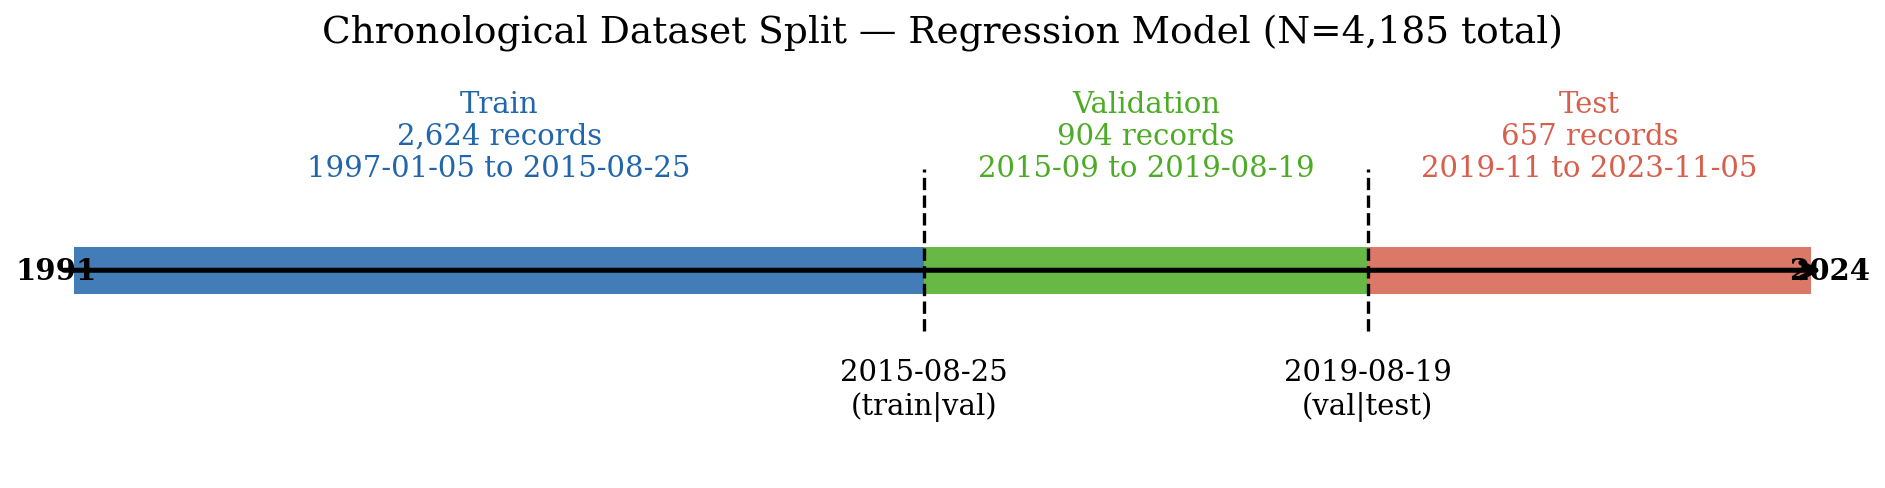
\includegraphics[width=\columnwidth]{figures/fig_chronological_split.png}
  \caption{Chronological dataset split for the regression model.
           Boundaries are determined by 70\,\%/85\,\% quantiles of
           unique observation dates; no station-date overlaps
           exist across partitions.}
  \label{fig:splits}
\end{figure}

\emph{Split audit}: Regression uses 2,624/904/657 records
(70\,\%/15\,\%/15\,\% unique dates); classification purges 113
boundary transitions ($\texttt{next\_date} \le \texttt{split\_end}$),
yielding 2,569/846/657 records. Both test on identical 657 records.

\subsection{Uncertainty Estimation}

Point-prediction uncertainty is evaluated via observation-level
empirical \textbf{bootstrap resampling} (i.i.d., 1,000 iterations, seed 42)
on the 657 test records, yielding empirical 95\% confidence
intervals of [1.77, 2.10]\,m for MAE, [2.61, 3.32]\,m for RMSE, and
[0.423, 0.639] for R$^2$. Resampling captures test variance without
assuming block temporal structure or epistemic uncertainty.

\subsection{Feature Importance Method}

Feature importance is computed by \textbf{permutation importance}
on the validation set (5 repetitions, random seed 42).
Importance is defined as the decrease in R$^2$ when each feature
column is randomly shuffled.
Negative values indicate features whose permutation slightly
improves performance (noise features); these are reported
transparently rather than suppressed.

\subsection{Baselines}

\textbf{Regression baselines} evaluated on the same 657 test records:
\begin{itemize}\setlength{\itemsep}{1pt}\setlength{\parskip}{0pt}
  \item \textit{Mean-target}: predicts the training-set mean GWL
        for every observation.
  \item \textit{Persistence}: predicts the current observed GWL
        as the next GWL (\emph{no-change} model).
\end{itemize}

\textbf{Classification baselines}:
\begin{itemize}\setlength{\itemsep}{1pt}\setlength{\parskip}{0pt}
  \item \textit{Majority-class}: always predicts ``No~Depletion''.
  \item \textit{Stratified dummy}: samples from the training-set
        class distribution (seed 42).
\end{itemize}

% ------------------------------------------------------------------
\section{Results}
\label{sec:results}
% ------------------------------------------------------------------

All metrics reported here are computed from saved prediction
artefacts (\texttt{models/test\_predictions.csv} and
\texttt{models/risk\_test\_predictions.csv}) on the chronologically
held-out test set (657 records, November 2019 -- November 2023).

\subsection{Regression Results}

Table~\ref{tab:reg} shows test-set performance.
The HistGBT model reduces MAE by 43.4\% relative to the mean-target
baseline and by 9.8\% relative to the persistence baseline.
The R$^2$ of 0.547 indicates that roughly 55\% of GWL variance in
the test period is explained by the model.
The relatively modest R$^2$ reflects the wide 40--200-day prediction
horizon and the inherent variability of manually monitored sparse
wells.

\begin{table}[h]
\caption{Regression Test-Set Performance (N\,=\,657, Nov~2019--Nov~2023)}
\label{tab:reg}
\centering
\footnotesize
\begin{tabular}{lccc}
\toprule
\textbf{Model} & \textbf{MAE (m)} & \textbf{RMSE (m)} & \textbf{R$^2$} \\
\midrule
Mean-target baseline & 3.43 & 4.39 & --- \\
Persistence baseline & 2.15 & 3.39 & --- \\
\textbf{HistGBT (ours)} & \textbf{1.94} & \textbf{2.96} & \textbf{0.547} \\
\bottomrule
\multicolumn{4}{l}{\footnotesize All metrics computed from saved artefacts.} \\
\multicolumn{4}{l}{\footnotesize Units: metres below ground level (mbgl).} \\
\end{tabular}
\end{table}

Fig.~\ref{fig:scatter} shows the actual-versus-predicted scatter
plot and the residual distribution.
The model tends to underpredict at extreme high depths
($>$\,15\,mbgl), reflecting the scarcity of such observations in
the training period.

\begin{figure}[t]
  \centering
  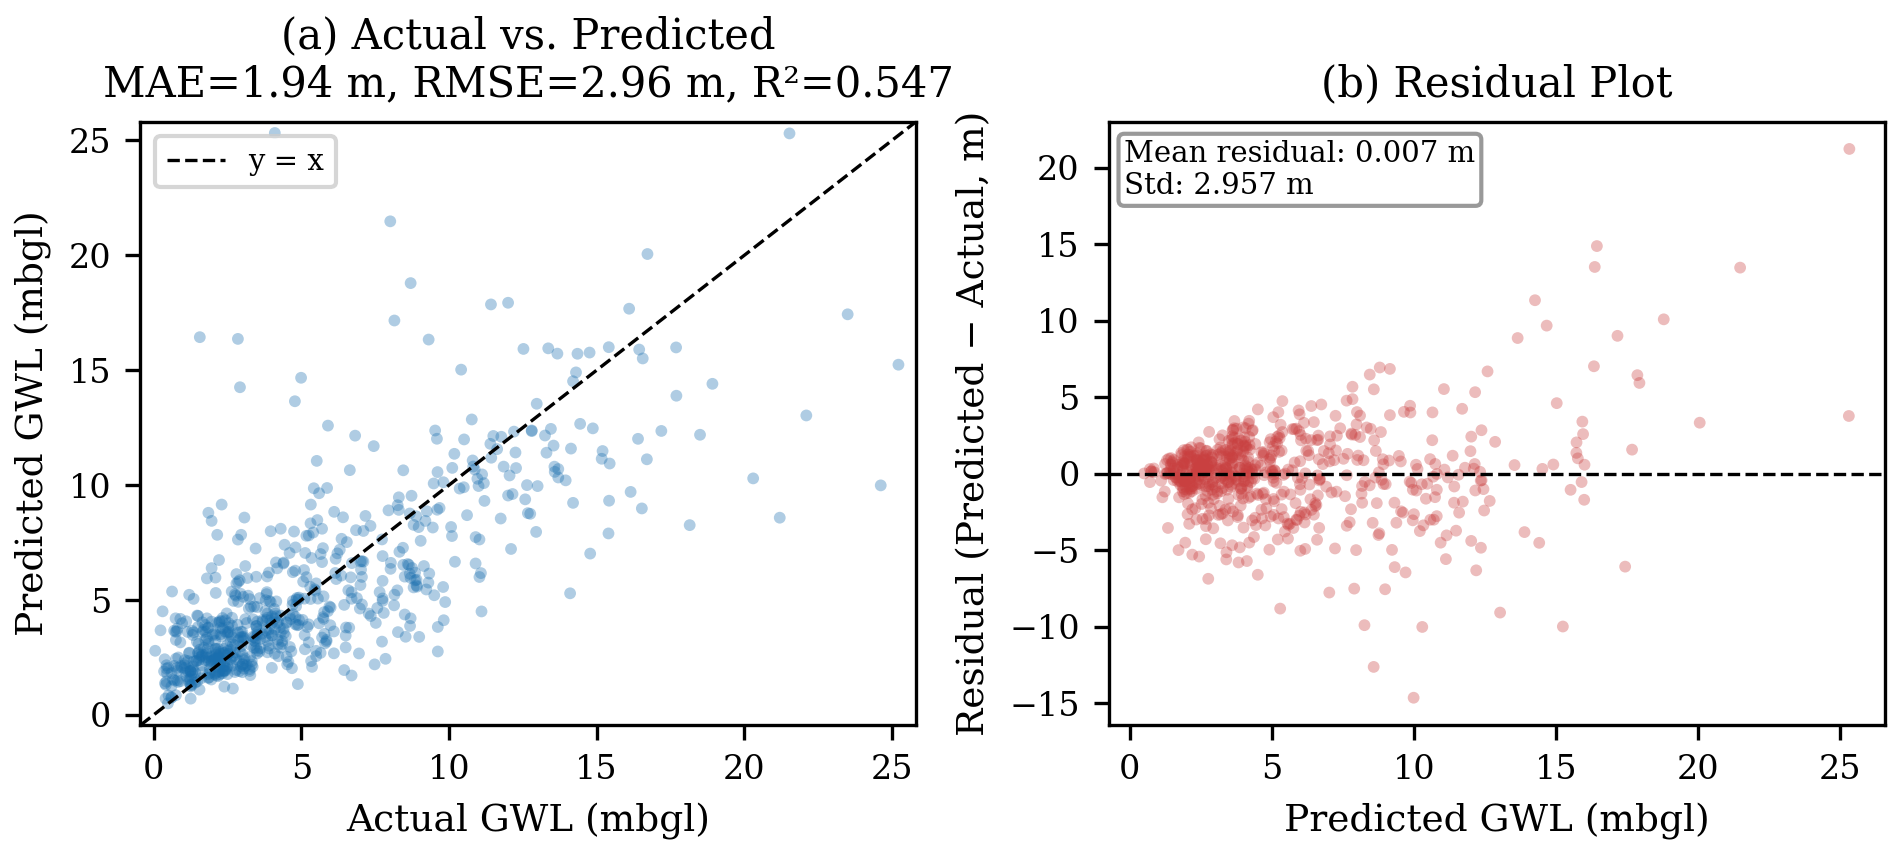
\includegraphics[width=0.66\columnwidth]{figures/fig_regression_scatter_residual.png}
  \caption{Regression results on the held-out test set (N\,=\,657).
           (a) Actual vs.\ predicted GWL (mbgl) with y=x reference.
           (b) Residual plot; mean residual $-0.01$\,m indicates
           negligible systematic bias.}
  \label{fig:scatter}
\end{figure}

\begin{figure}[t]
  \centering
  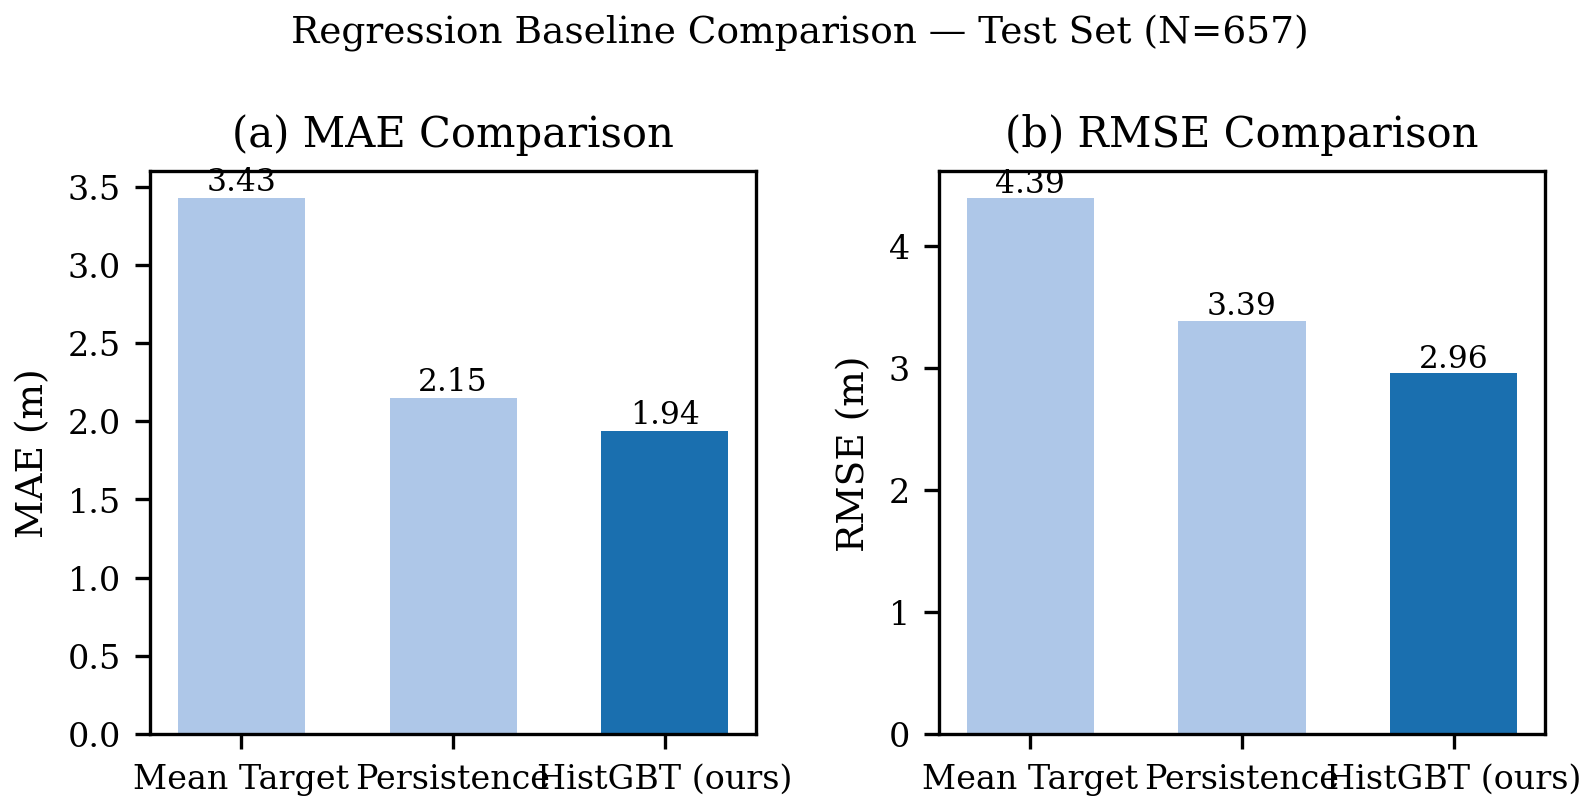
\includegraphics[width=0.56\columnwidth]{figures/fig_baseline_comparison.png}
  \caption{Regression baseline comparison on the test set.
           HistGBT reduces MAE by 43\% vs.\ mean-target baseline
           and by 10\% vs.\ the persistence baseline.}
  \label{fig:baselines}
\end{figure}

\subsection{Classification Results}

Table~\ref{tab:cls} reports classification performance for the
Random Forest model.
The model outperforms both baselines on accuracy and macro-F1.
High-risk classification (F1\,=\,0.33) is the weakest, reflecting
the class imbalance (only 80 test examples, 12.2\%) and
the difficulty of detecting extreme depletion events in quarterly
data.

\begin{table}[h]
\caption{Classification Test-Set Performance (N\,=\,657, Nov~2019--Nov~2023)}
\label{tab:cls}
\centering
\footnotesize
\begin{tabular}{lccc}
\toprule
\textbf{Model} & \textbf{Accuracy} & \textbf{Macro F1} & \textbf{Wt.\ F1} \\
\midrule
Majority-class baseline & 0.458 & 0.157 & --- \\
Stratified dummy (seed=42) & 0.304 & 0.253 & --- \\
\textbf{Random Forest (ours)} & \textbf{0.528} & \textbf{0.457} & \textbf{0.529} \\
\bottomrule
\end{tabular}
\end{table}

\begin{table}[h]
\caption{Per-Class Performance --- Random Forest (Test Set)}
\label{tab:perclass}
\centering
\footnotesize
\begin{tabular}{lcccc}
\toprule
\textbf{Class} & \textbf{Prec.} & \textbf{Recall} &
\textbf{F1} & \textbf{Support} \\
\midrule
No Depletion & 0.70 & 0.69 & 0.70 & 301 \\
Low          & 0.38 & 0.39 & 0.38 & 129 \\
Moderate     & 0.42 & 0.42 & 0.42 & 147 \\
High         & 0.33 & 0.33 & 0.33 &  80 \\
\midrule
Macro avg    & 0.46 & 0.46 & 0.46 & 657 \\
Weighted avg & 0.53 & 0.53 & 0.53 & 657 \\
\bottomrule
\end{tabular}
\end{table}

Fig.~\ref{fig:cm} presents the confusion matrix (counts and
row-normalised fractions).
The dominant error mode for No~Depletion (301 actual) is
misclassification as Moderate (34 cases) or High (30 cases),
which would constitute false alarms in a screening application.
For High depletion (80 actual), 48 cases are misclassified---32 as
Moderate and 16 as No~Depletion---representing missed detections
that would be operationally consequential.

\begin{figure}[t]
  \centering
  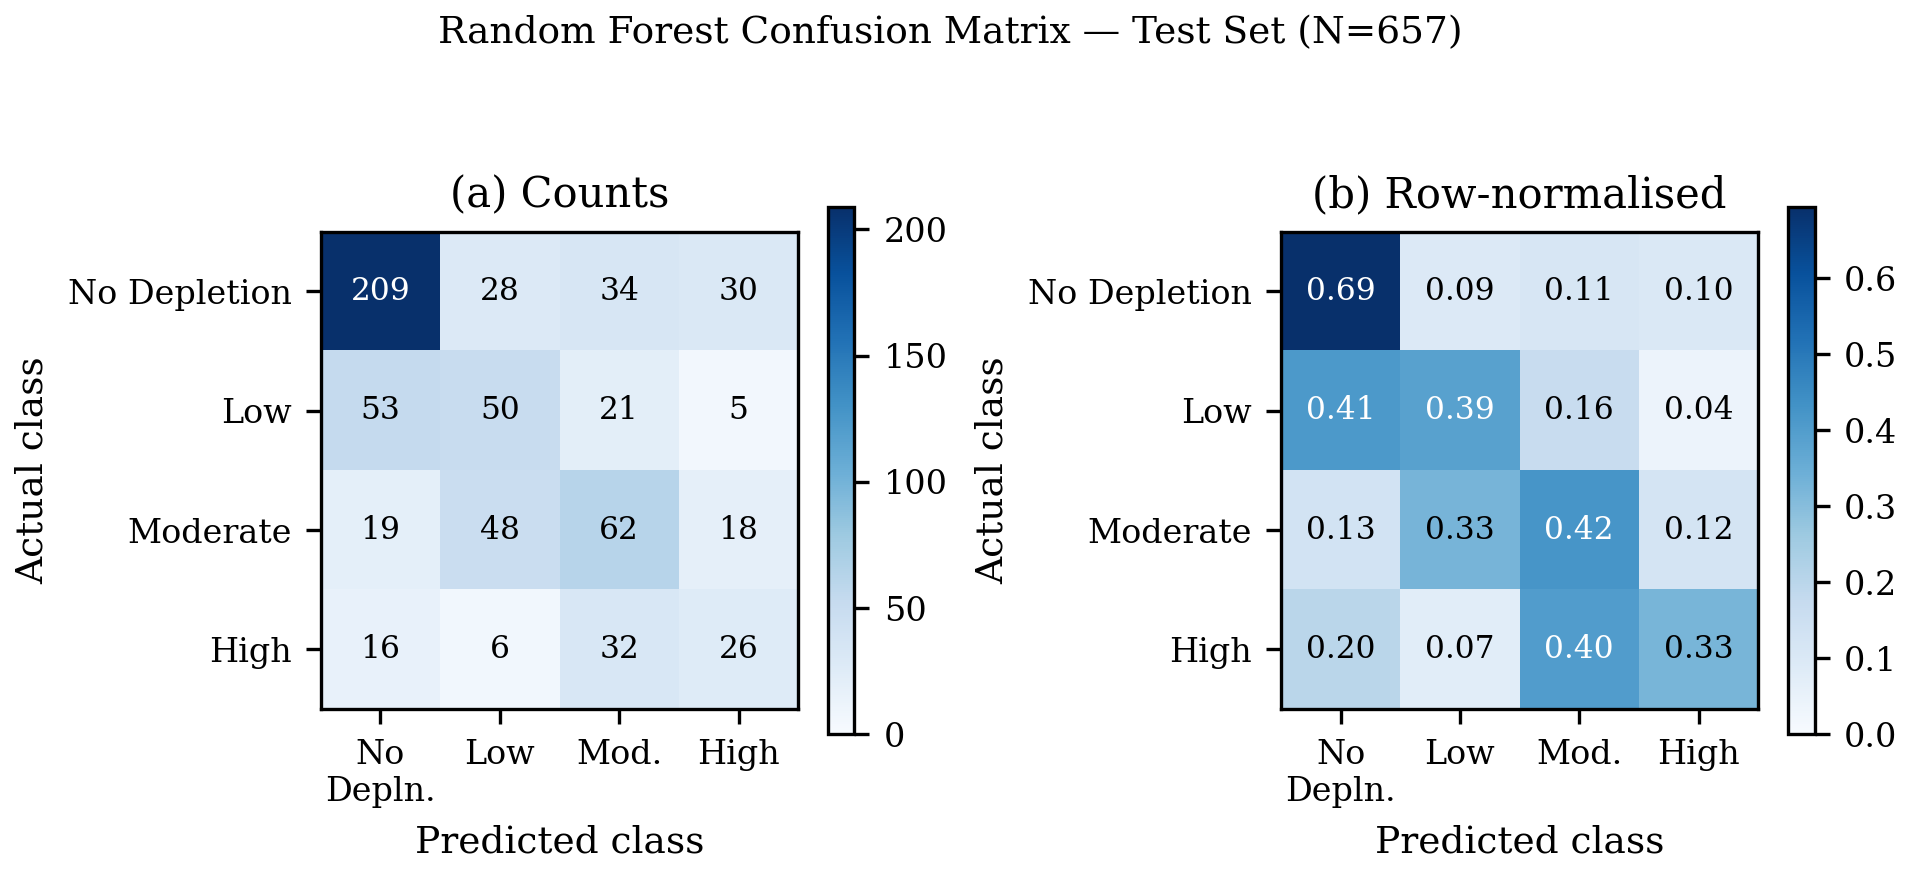
\includegraphics[width=0.66\columnwidth]{figures/fig_confusion_matrix.png}
  \caption{Random Forest confusion matrix --- test set (N\,=\,657).
           (a) Raw counts; (b) row-normalised fractions.
           Diagonal entries represent correct classifications.}
  \label{fig:cm}
\end{figure}

\begin{figure}[t]
  \centering
  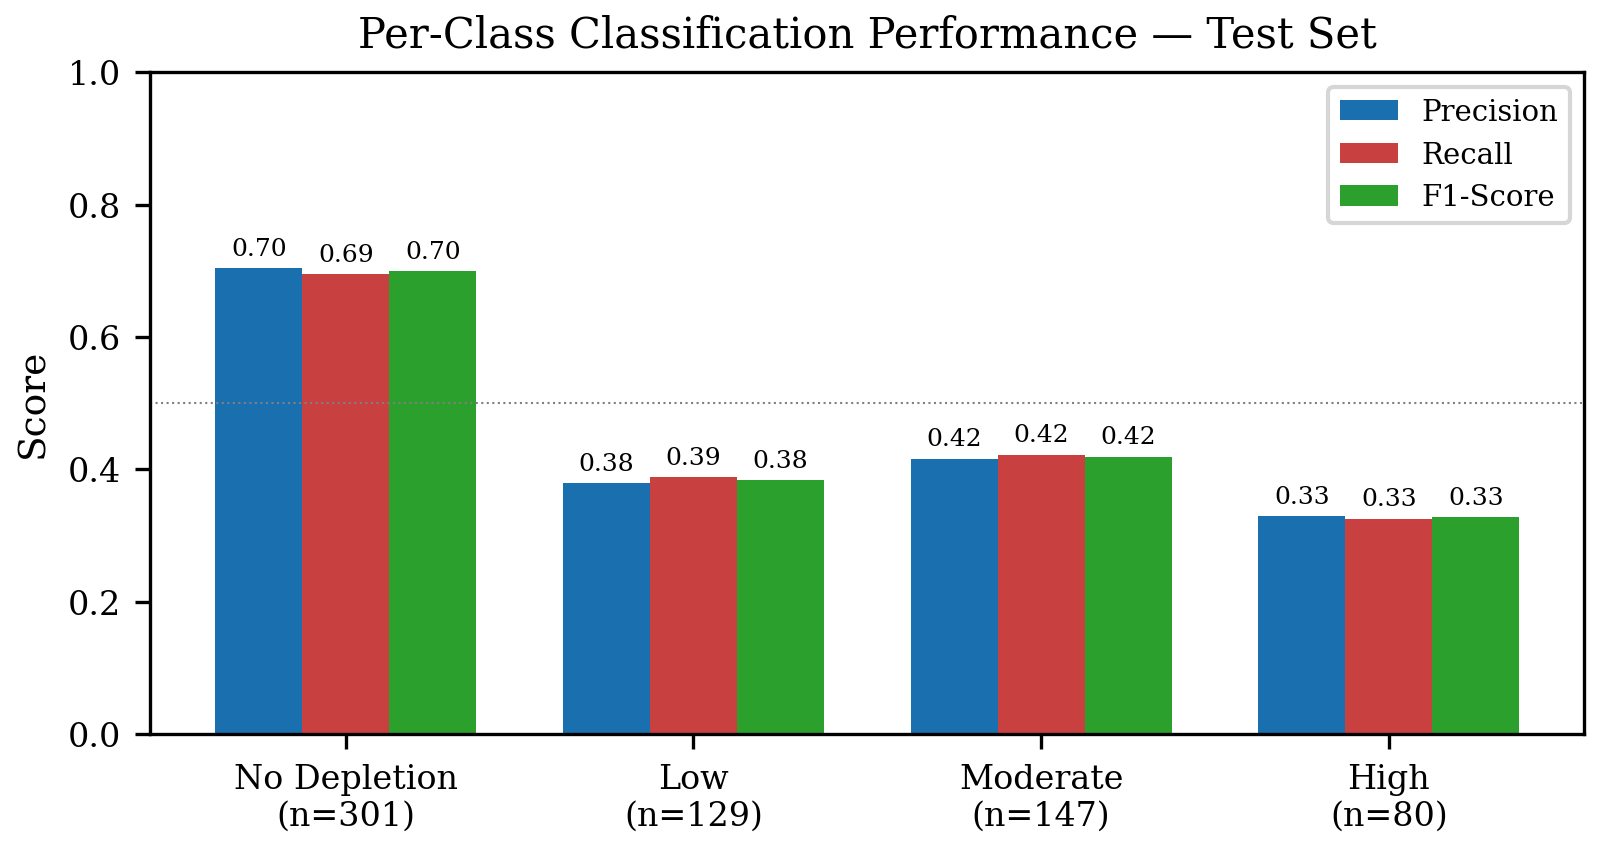
\includegraphics[width=0.56\columnwidth]{figures/fig_class_performance.png}
  \caption{Per-class precision, recall, and F1-score for the
           Random Forest classifier.
           Support counts shown below class labels.}
  \label{fig:classperf}
\end{figure}

\subsection{Feature Importance}

Permutation importance (Fig.~\ref{fig:fi}) identifies
current GWL (\texttt{groundwater\_level\_m}, importance 0.592)
and the 4-observation rolling mean (\texttt{gw\_rolling\_mean\_4},
0.328) as the most influential features.
Cyclical month encoding and station historical mean follow.
Short-window rainfall features (7-day: 0.011) carry modest positive
importance, while longer-window rainfall features (90, 180, 365 days)
show near-zero or slightly negative importance on the validation set.
This does not imply that long-term rainfall is physically
unimportant; it may reflect collinearity with GWL
history, irregular rainfall data coverage, or the limited
discriminative power of district-averaged rainfall at the
station scale.
Caution is warranted in interpreting negative importance values as
evidence of harmful features.

\begin{figure}[t]
  \centering
  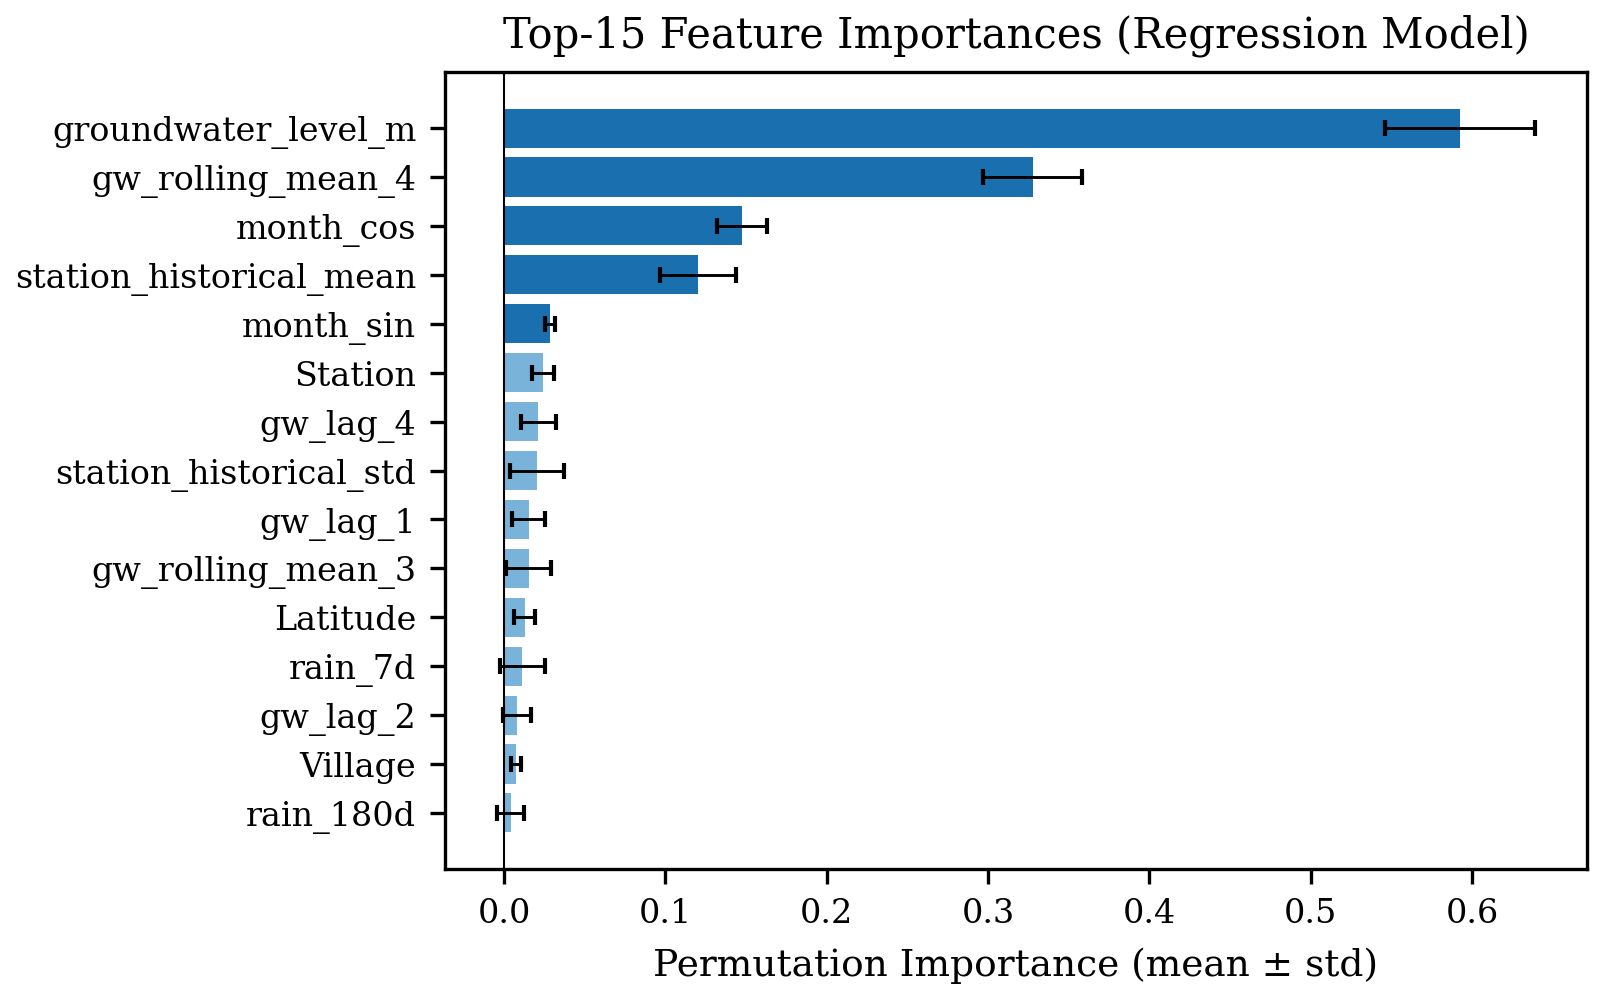
\includegraphics[width=0.42\columnwidth]{figures/fig_feature_importance.png}
  \caption{Top-15 permutation feature importances (mean\,$\pm$\,std)
           for the regression model.
           Importance is defined as the decrease in R$^2$ upon
           random permutation of each feature.}
  \label{fig:fi}
\end{figure}

% ------------------------------------------------------------------
\section{Discussion, Limitations, and Threats to Validity}
\label{sec:discussion}
% ------------------------------------------------------------------

\subsection{Key Findings}

The HistGBT regressor meaningfully reduces prediction error relative
to both the mean-target and persistence baselines, suggesting that
GWL history and station characteristics carry predictive signal
beyond a no-change assumption.
The four-class depletion classifier achieves modest but above-chance
performance, outperforming both baselines on macro-F1 by factors of
2.9$\times$ and 1.8$\times$ respectively.

\subsection{Limitations}

\begin{enumerate}\setlength{\itemsep}{0pt}\setlength{\parskip}{0pt}
  \item \textbf{Sparse station network.}
        92 manual observation wells across Mysuru district
        (approximately 6,645~km$^2$) provide an average density
        of roughly 1 station per 72~km$^2$.
        Unmonitored areas, particularly those with deep confined
        aquifers or significant extraction, are not represented.

  \item \textbf{Variable prediction horizon.}
        The model predicts one observation ahead regardless of
        the inter-observation gap (40--200 days).
        Fixed-metre risk thresholds conflate different rates of
        change across intervals; hydrogeologically, a 3-m change
        over 40 days is far more alarming than the same change
        over 200 days.

  \item \textbf{Missing rainfall.}
        Gaps in the NWDP daily rainfall series (including December 2023)
        mean that rolling accumulation features carry partial-window
        uncertainty near gap boundaries.
        Missing rainfall is retained as \texttt{NaN}
        (not imputed to zero), but propagation through rolling
        windows with \texttt{min\_periods=1} means that some
        features silently cover fewer days than their window name
        implies.

  \item \textbf{Empirical risk thresholds.}
        The Low/Moderate/High boundaries (1 and 3~m) are heuristic
        and not validated against CGWB's official
        semi-critical/critical/over-exploited classifications,
        which are based on multi-year extraction-recharge balances
        rather than observation-to-observation changes.

  \item \textbf{High-risk detection.}
        F1 of 0.33 for the High class means that roughly two in three
        High-risk events are not correctly identified.
        The model is not reliable for early warning of extreme
        depletion without further improvement.

  \item \textbf{Rainfall feature influence.}
        Most rainfall permutation-importance values are near zero
        or negative, particularly for long windows.
        This may reflect collinearity, district-averaged aggregation
        losing local signal, or the lagged relationship between
        rainfall and shallow versus deep aquifer response.

  \item \textbf{No temporal cross-validation.}
        A single temporal holdout is used.
        Walk-forward cross-validation would provide more robust
        performance estimates but was not feasible given dataset size.

  \item \textbf{Dashboard is exploratory.}
        The web dashboard presents model outputs for visual
        exploration only.
        It does not provide calibrated probabilities, uncertainty
        bands, or validation against real-time measurements.
        It is not suitable for operational groundwater management
        decisions.
\end{enumerate}

\subsection{Threats to Validity}

\textbf{Internal validity}: Chronological partitioning prevents temporal leakage; features strictly precede prediction dates.
\textbf{External validity}: Findings may not generalize to disparate lithologies or non-quarterly monitoring protocols.
\textbf{Construct validity}: The horizon reflects monitoring intervals rather than fixed operational lead times; decisions depend on known visit schedules.

\section{Conclusion and Future Work}
\label{sec:conclusion}
% ------------------------------------------------------------------

We presented an exploratory machine-learning system for GWL
prediction and depletion-risk classification at CGWB monitoring
wells in Mysuru district, Karnataka.
Using 27+ years of quarterly observations from 92 stations and
district-averaged NWDP daily rainfall (ingested from local snapshots),
a Historical Gradient Boosting Regressor achieves MAE\,=\,1.94\,m
and R$^2$\,=\,0.547 on 657 chronologically held-out test records
(2019--2023), reducing prediction error by 43\% versus the mean baseline.
A companion Random Forest classifier achieves 52.8\% accuracy and
macro-F1 of 0.457 for four-class depletion severity, outperforming
both majority-class and stratified baselines.

Key limitations include variable prediction horizons with
fixed-metre risk thresholds, sparse monitoring coverage, partial
rainfall data, and low recall on the rare High-risk class.
The system is presented as an exploratory decision-support
prototype rather than an operational early-warning tool.
Future priorities include: (1) calibrating empirical risk boundaries against statutory CGWB extraction assessments; (2) incorporating hydrogeological lithology covariates; (3) exploring conformal uncertainty intervals; (4) evaluating interval-normalized drawdown rates; and (5) assessing transferability across adjacent peninsular river basins.

% ------------------------------------------------------------------
% REFERENCES
% ------------------------------------------------------------------

% ------------------------------------------------------------------
\textbf{Data and Code Availability.}
% ------------------------------------------------------------------
The complete machine-learning pipelines, verification scripts,
evaluation summaries, and full-stack web application are available
at \url{https://github.com/Mohammed-Sadiq-Shariff/groundwater-depletion-risk-prediction}
(commit \texttt{0272a78}, accessed 20~October~2026).
Groundwater and rainfall records are hosted on the National
Water Data Portal (NWDP).

\bibliographystyle{IEEEtran}
\bibliography{references}

\end{document}
